\documentclass[a4paper,12pt]{article}
\usepackage[utf8]{inputenc}
\usepackage[T1]{fontenc}
\usepackage{graphicx}
\usepackage{hyperref}
\usepackage{listings}
\usepackage{amsmath}
\usepackage{float}
\usepackage{geometry}
\usepackage{polski}
\usepackage{color}

\geometry{margin=1in}

\title{Sprawozdanie z laboratorium 3}
\author{Mikołaj Kubś 272662}
\date{\today}

\begin{document}

\maketitle

\section{Cel zadania}

Celem zadania jest stworzenie prostej aplikacja PWA z wykorzystaniem HTML, CSS i JS. Kolejnym krokiem był deployment i testy funkcjonalności.

\subsection{Wprowadzenie}

Progressive Web App to aplikacja internetowa uruchamiana tak jak zwykła strona internetowa, ale
umożliwiająca stworzenie wrażenia działania jak natywna aplikacja mobilna (lub aplikacja
desktopowa).

\subsection{Tworzenie aplikacja PWA z wykorzystaniem HTML, JS i CSS}

\subsubsection{Kod HTML}
Plik \texttt{index.html} definiuje prosty kod HTML aplikacji:

\begin{figure}[H]
    \centering
    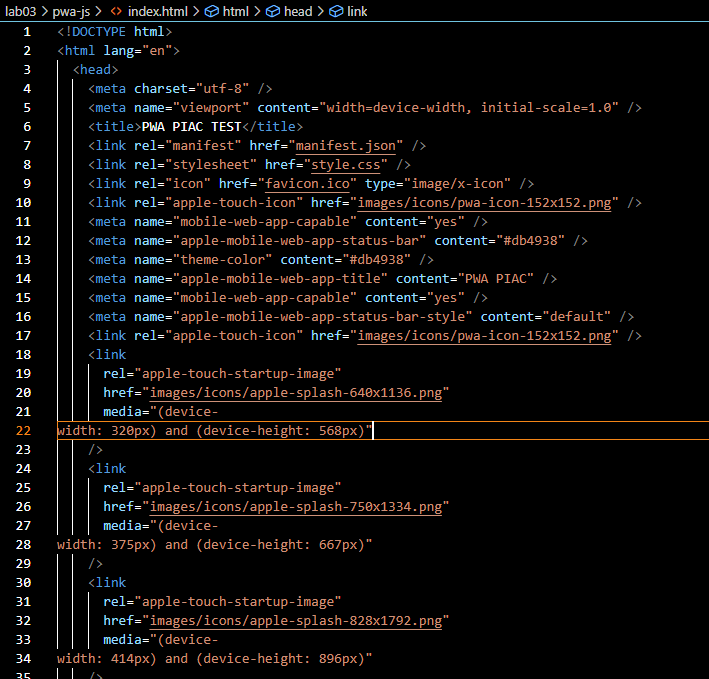
\includegraphics[width=1\textwidth]{images/index_html.png}
    \caption{Kod index.html}
\end{figure}

\subsubsection{Stylizacja CSS}
Plik \texttt{style.css} definiuje kaskadowe arkusze stylów:

\begin{figure}[H]
    \centering
    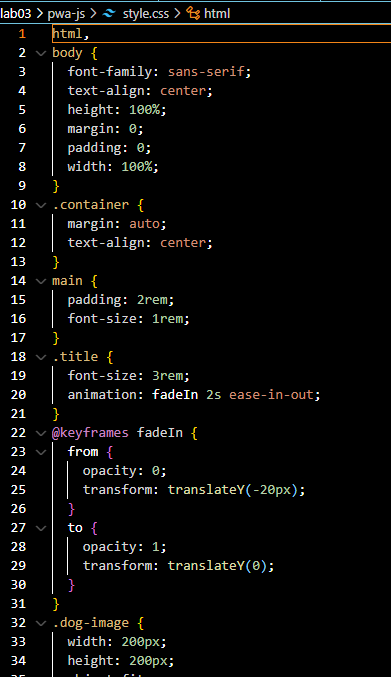
\includegraphics[width=1\textwidth]{images/css.png}
    \caption{Fragment kodu style.css}
\end{figure}

\subsubsection{Kod JavaScript}
Plik \texttt{router.js} zarządza nawigacją w aplikacji SPA:

\begin{figure}[H]
    \centering
    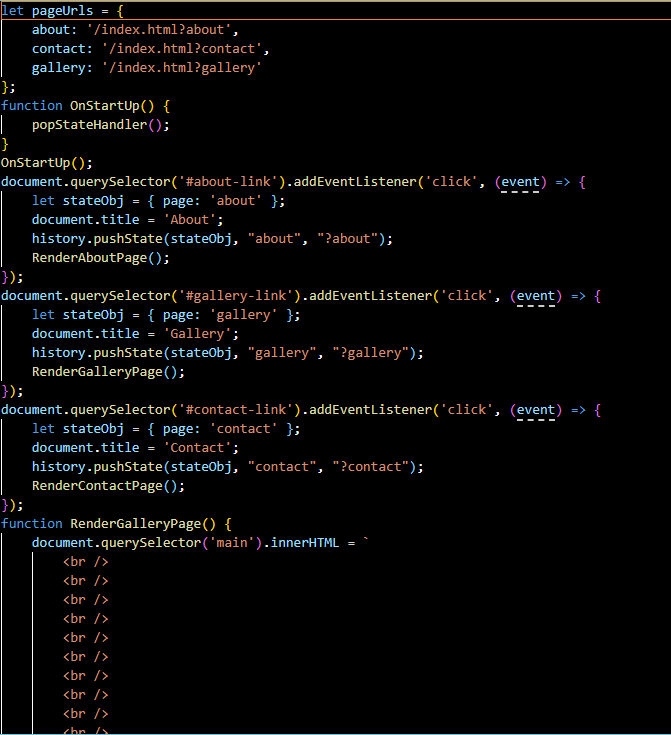
\includegraphics[width=1\textwidth]{images/js.png}
    \caption{Fragment kodu router.js}
\end{figure}

\end{document}
